% Chapter Template

\chapter{Results} % Main chapter title

\label{Methodology} % Change X to a consecutive number; for referencing this chapter elsewhere, use \ref{ChapterX}

\lhead{Chapter 5. \emph{Results}} % Change X to a consecutive number; this is for the header on each page - perhaps a shortened title

%----------------------------------------------------------------------------------------
%	SECTION 1
%----------------------------------------------------------------------------------------

\section{Simulation}
We ran \srthree which was described in chapter \ref{soft}. Our aim was to simulate $10^{4}$ photons produced by a proton beam at 7 TeV energy. This amount of photons was used to balance a large enough number to present accurate statistical results and the amount of available computing time, but because of technical challenges mentioned in subsection \ref{lxplus}, we divided the simulation into several simulations with a much smaller number of photons, there were simulations with 10, 20 and 50 photons each, which we can join together because photons do not interact with each other.



%-----------------------------------
%	SUBSECTION 1
%-----------------------------------
\subsection{SMIF}
The SMIF used to run this simulations used the following parameters:
\begin{itemize}
\item The wall file describing the vacuum chamber with a sawtooth pattern, of a series of 30 $\mu$m high steps at adistance of 500 $\mu$m in the longitudinal direction, which is on the horizontal. (sawtoohTEST.wall). The transversal section of the beam screen is shown in Figure \ref{fig:xy}.

\begin{figure}
	\centering
  \begin{minipage}{\textwidth}
  	\centering
   	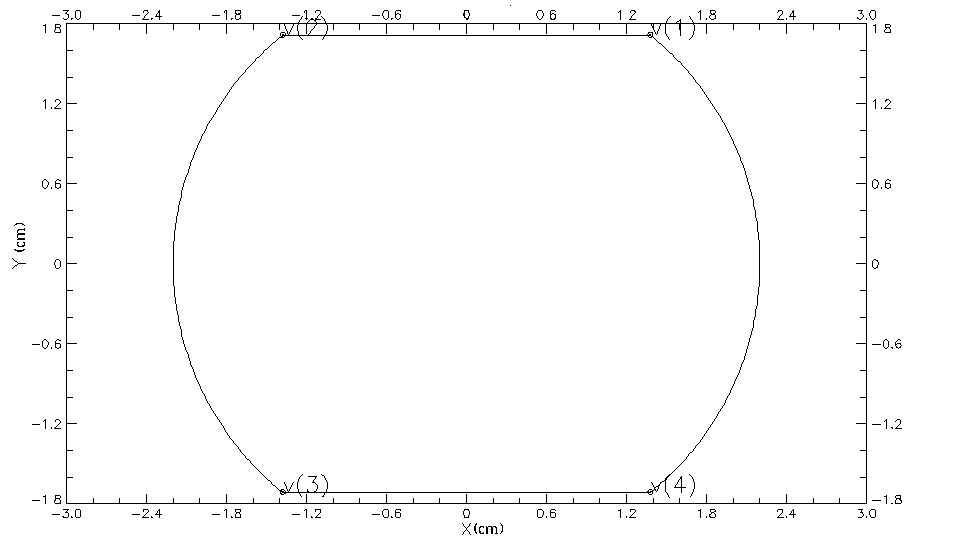
\includegraphics[width=5.5in]{Pictures/transsect.jpg}
  		\caption{\label{fig:xy}
   			Transversal section of the beam screen in the cold arcs. }
   			\footnotesize{Image plotted with \srthree}
   \end{minipage}
\end{figure}
\item The lattice file which contains the version 6.5 of the LHC was employed. (V6.5.out.bmad)
\item The starting element was set to be 142 and the ending element 146. All elements inside that range are bending dipoles.
\item The photon direction was set to be positive wich means a forward generation.
\item The number of photons varied between 10, 20 and 50.
\item The seed for the random number generator was set to be the system clock.
\item A custom reflectivity table was used. (reflectivity.table.C.CU.dat). This table assumes a carbon layer of 10 nm on a copper substrate. For this table the probability of reflection ($P_{\textrm{reflect}}$) was taken from the LBNL X-ray database\cite{lbnl}.
\end{itemize} 

%-----------------------------------
%	SUBSECTION 2
%-----------------------------------

\subsection{SMOF}
After all simulations were run through the batch system the results were concatenated into a single file containing a single table with the information of 9,227 photons that where generated, and absorbed by the beam screen between sections 142 and 146.


%----------------------------------------------------------------------------------------
%	SECTION 2
%----------------------------------------------------------------------------------------
\subsection{Secondary Simulation}
In order to have data to compare to the data we obtained, we ran a single simulation featuring $10^4$ photons using the same parameters except the sawtooth pattern of the wall file. In other words we simulated with the same parameters but with a smooth beam pipe. We kept the first 9,227 photons just to have the same number of photons in both simulations.

\subsection{Analysis}
In both simulations all photons were absorbed in the last element analyzed (bending magnet 146) with no rebounds. The exact position where photons were absorbed are shown in Figure \ref{fig:s}. Figure \ref{fig:s} shows an histogram of photons absorbed versus the position on the s axis, The ones from the sawtooth pattern simulation is are shown in red, and the ones from the smooth surface simulation in blue.
\begin{figure}%[ht]
%\centering % used for centering table
 % \begin{minipage}{\textwidth}
  	\centering
   	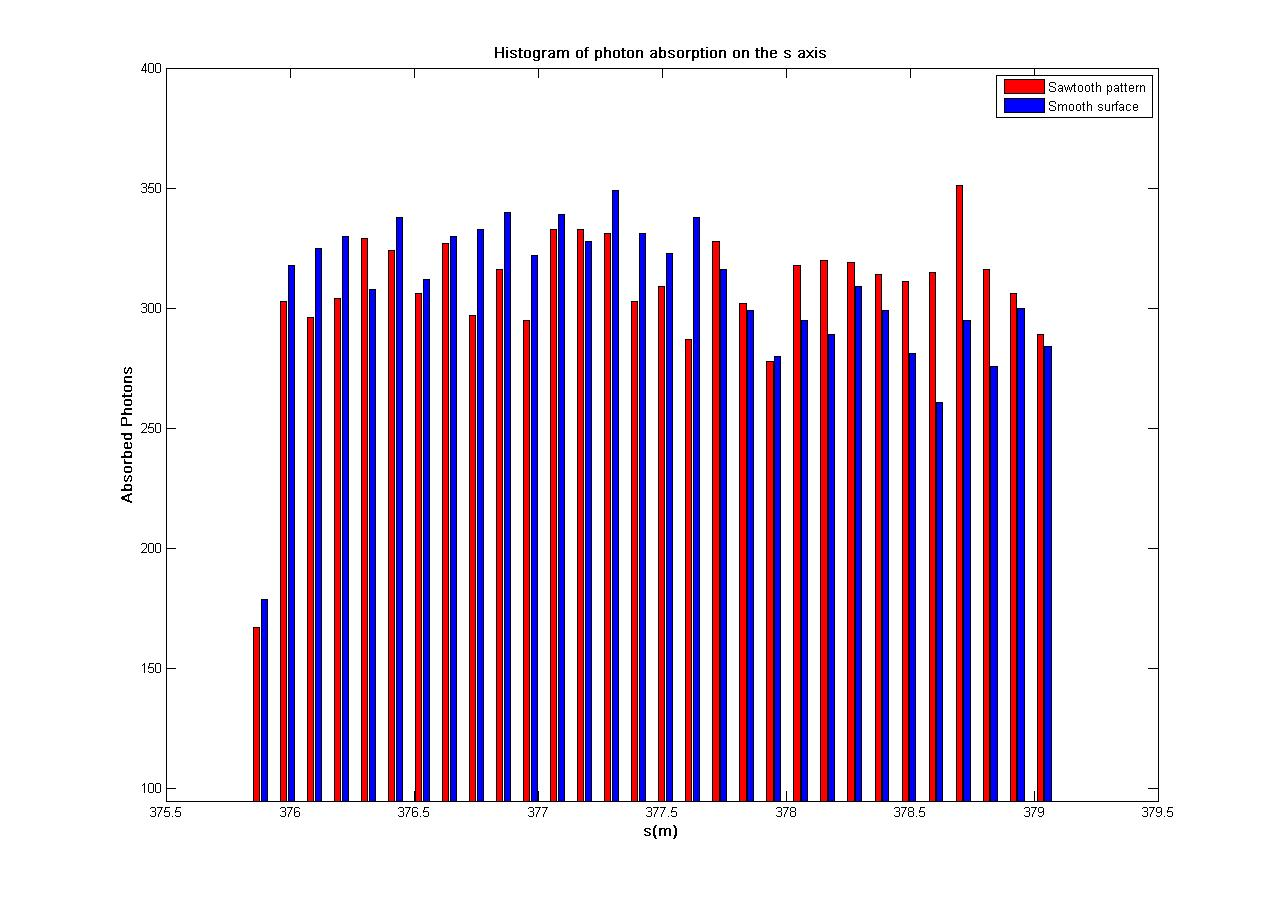
\includegraphics[width=6.5in, height=.65\textheight]{Graficas/nuevas/sbarras.jpg}
  		\caption{\label{fig:s}
   			Position on the s axis where photons were absorbed.}
%   			\footnotesize{Image plotted with \srthree}
  % \end{minipage}
 \end{figure}


The energies at which photons were absorbed are shown in Figure \ref{fig:energia}. It shows in blue the results for the primary simulation and in red the result for the secondary simulation. The mean energy from all photons absorbed by the sawtooth pattern is 27.109 eV and 27.113 for the smooth surface.  

\begin{figure}%[ht]
%\centering % used for centering table
%  \begin{minipage}{\textwidth}
  	\centering
   	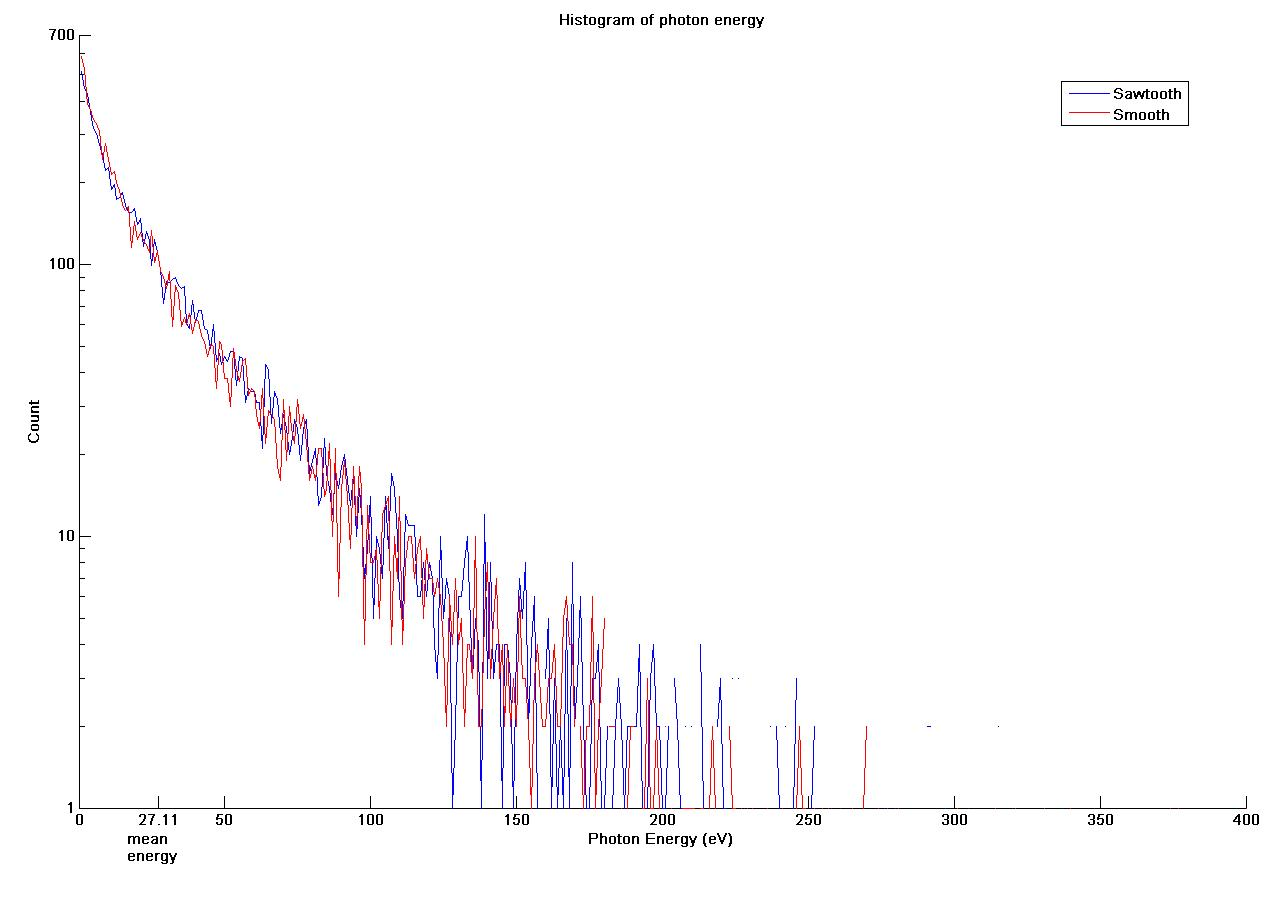
\includegraphics[width=6.5in, height=.65\textheight]{Graficas/nuevas/energias.jpg}
  		\caption{\label{fig:energia}
   			Energy of absorbed photons. }
%   			\footnotesize{Image plotted with \srthree}
 %  \end{minipage}
\end{figure}



An histogram for the position X-Y where photons were absorbed are shown in Figure \ref{fig:xy} for the main simulation and Figure \ref{fig:xyplana} for the smooth beam pipe. 
\begin{figure}

%\centering % used for centering table
%  \begin{minipage}{\textwidth}
  	\centering
   	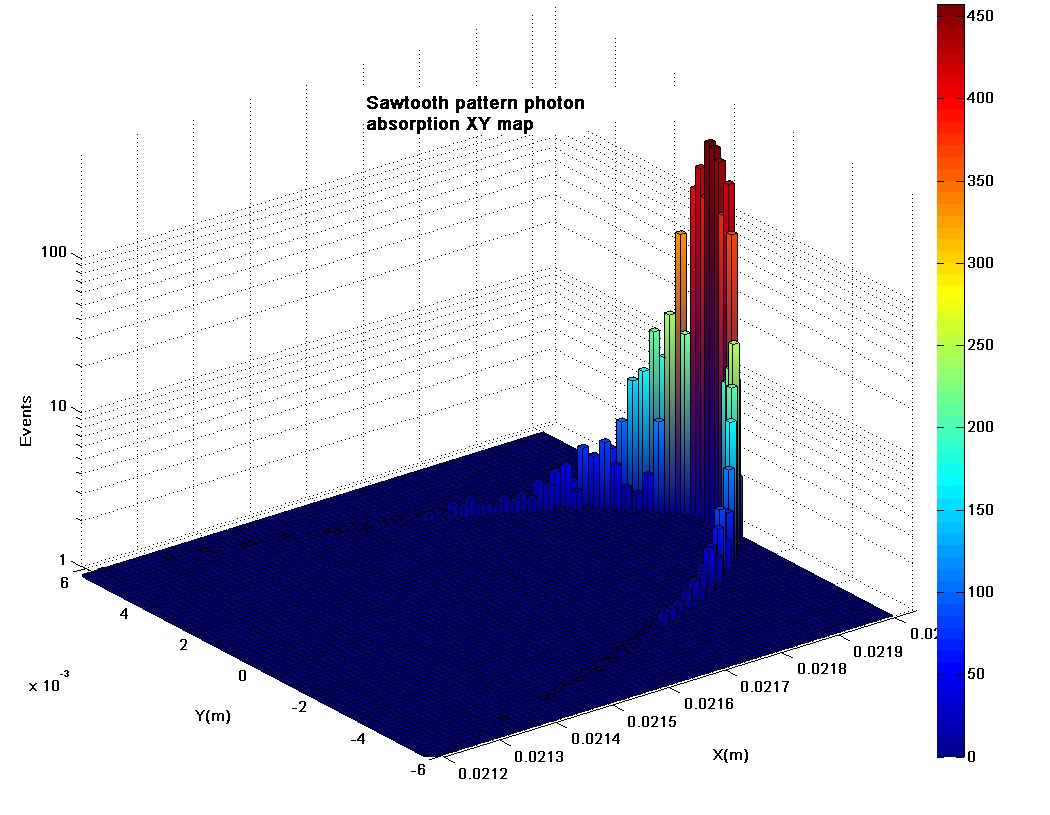
\includegraphics[height=.45\textheight]{Graficas/nuevas/xy.jpg}
  		\caption{\label{fig:xy}
   			 X-Y absorption points for the sawtooth pattern beam screen.}
%   			\footnotesize{Image plotted with \srthree}
 %  \end{minipage}
\end{figure}   

 \begin{figure}
 
  % \begin{minipage}{\textwidth}
  	\centering
   	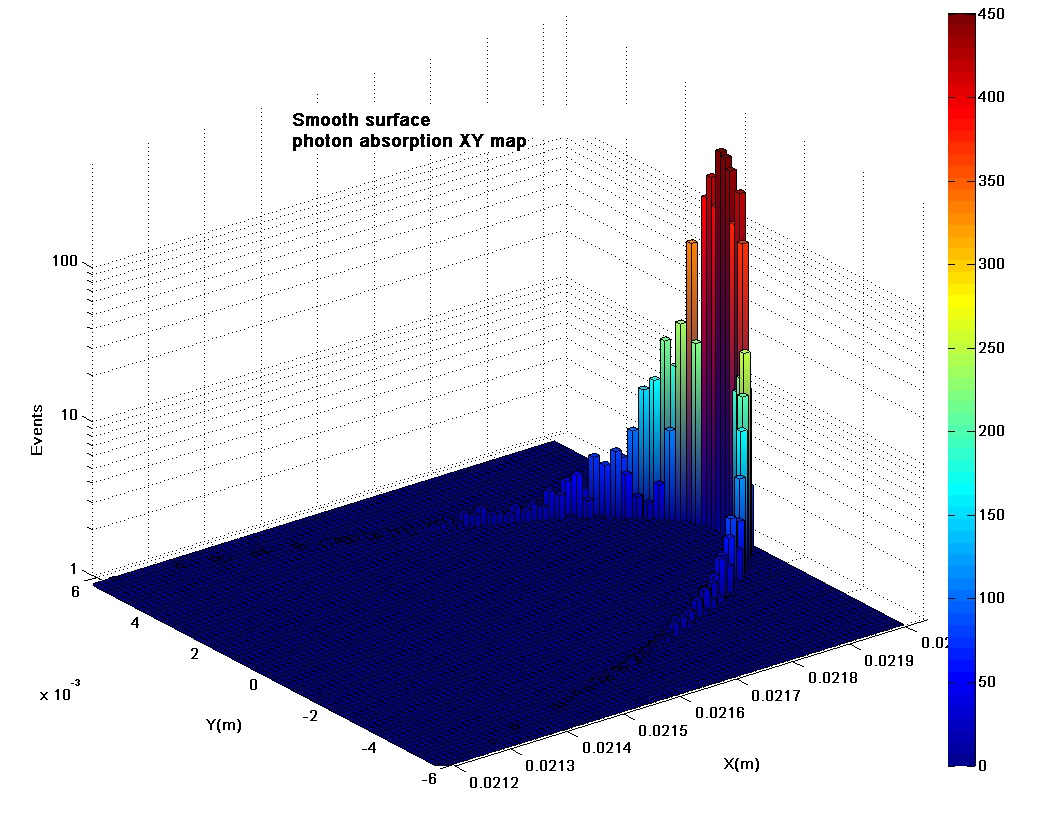
\includegraphics[height=.45\textheight]{Graficas/nuevas/smoothxy.jpg}
  		\caption{\label{fig:xyplana}
   			X-Y absorption points for the smooth surface beam screen.}
%   			\footnotesize{Image plotted with \srthree}
%\end{minipage}
%\label{comp:3} % is used to refer this table in the text
\end{figure}



